\begin{center}
	\textbf{\LARGE{Metoda končnih elementov, ki minimizira kvadrat ostanka aproksimacije (\texttt{LSFEM})}}\\[0.25cm]
	\large{Seminarska naloga pri Naprednih numeričnih metodah}\\[0.7cm]
\end{center}

Numerično reševanje parcialnih diferencialnih enačb (\texttt{PDE}) je zaradi pomanjkanja vsestranskega algoritma še zmeraj bolj umetnost kot ustaljena znanost \cite{JiangB-LSFEM}. Pri zapletenih problemih hitro prispemo do vznožja gore matematične teorije, ki je ni moč zaobiti. Zaradi množice različnih pristopov reševanja ter raztresene in neprijazno napisane literature, lahko le ugibamo, kako visoko se bomo na poti do prelaza morali povzpeti. Zapletenim problemom prostorske dinamike v:
\begin{center}
	\begin{tabular}[h]{lll}
		\tabitem dinamiki tekočin,\hspace{1cm}	&	\tabitem termodinamiki,\hspace{2.5cm}	&	\tabitem elektrodinamiki,\\
		\tabitem kvantni teoriji,	&	\tabitem splošni teoriji relativnosti,&	\\
	\end{tabular}
\end{center}
kjer naletimo na \texttt{PDE}, se tako tudi v višjem izobraževanju najraje izognemo. Metoda končnih elementov (\texttt{FEM}), ki minimizira kvadrat ostanka aproksimacije (\texttt{LSFEM} = Least Squares \texttt{FEM}), obeta razvoj vsestranskega algoritma za reševanje \texttt{PDE} in s tem približanje omenjenih problemov širšemu krogu raziskovalcev.

\section{Podlaga za temelje \texttt{LSFEM}}
Kadar obravnavamo prostorsko dinamiko (npr.\ tok tekočine), lahko fizični prostor modeliramo kot 1, 2 ali 3-mnogoterost. Temelje \texttt{LSFEM} bomo polagali na splošnem primeru $d$-mnogoterosti, za ponazoritev pa na njih sproti gradili konkretni 2D primer.

\begin{wrapfigure}{r}{5.5cm}
	\vspace{-0.3cm}
	\centering
	\captionsetup{type=figure}
	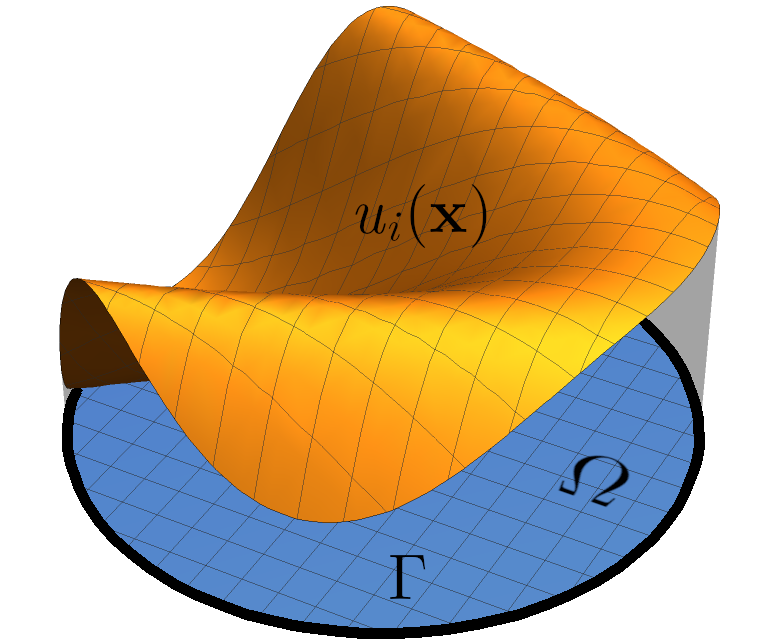
\includegraphics[width=5.5cm]{Slike/funkcijaInDomenaG}
	\caption{Domena $\Omega$, meja domene $\Gamma$ in komponenta rešitve $u_i(\mathbf{x})$.}
\label{fig:funkInDom}
\vspace{-2.6cm}
\end{wrapfigure}
Naj bo torej prizorišče dogajanja $d$-mnogoterost $\Omega$, opremljena s krajevnim vektorjem $\mathbf{x} = \{x_1, ..., x_d\}$. Pri reševanju sistema $m$ \texttt{PDE} iščemo nabor funkcij $\mathbf{u}(\mathbf{x}) =  \{u_1(\mathbf{x}), ..., u_m(\mathbf{x})\}$, ki v vsaki točki domene $\Omega$ zadosti sistemu \texttt{PDE}, na meji $\Gamma$ pa robnim pogojem (slika \ref{fig:funkInDom}). Konkretni primer bomo gradili na \textbf{sistemu Stokesovih enačb} za nestisljive tekočine v obliki \emph{u-p-$\omega$} (hitrost, tlak, vrtinčnost):\\[0.05cm]
\begin{minipage}{5.0cm}
\begin{IEEEeqnarray}{rl}
	\frac{\pd u}{\pd x} + \frac{\pd v}{\pd y} &= 0 \ , \label{eq:StokesDiv} \\[0.3cm]
	\frac{\pd p}{\pd x} + \frac{\pd \omega}{\pd y} &= f_1 \ ,
\end{IEEEeqnarray}
\end{minipage}
\begin{minipage}{5.3cm}
\begin{IEEEeqnarray}{rl}
	\frac{\pd p}{\pd y} - \frac{\pd \omega}{\pd x} &= f_2 \ , \\[0.3cm]
	\omega - \frac{\pd u}{\pd y} - \frac{\pd v}{\pd x} &= 0 \ . \label{eq:StokesCurl}
\end{IEEEeqnarray}
\end{minipage}\\[0.4cm]
To je le sistem stacionarnih Navier-Stokesovih enačb brez nelinearnih konvektivnih členov, ki jih moramo pri numeričnem reševanju linearizirati. Ker ta korak za ponazoritev \texttt{LSFEM} ni ključen, se mu na tak način izognemo. Kot zanimivost navržimo, da Stokesove enačbe opisujejo plazeče se tokove, pri katerih je konvekcija gibalne količine (zaradi gibanja) majhna v primerjavi z njeno difuzijo (zaradi viskoznosti). V enačbah ni časovnih odvisnosti (razen preko časovno odvisnih robnih pogojev), zato so takšni tokovi časovno obrnljivi: časovno obrnjena rešitev enačb je prav tako rešitev (slika \ref{fig:TaylorCouette}).

\begin{figure}[!ht]
	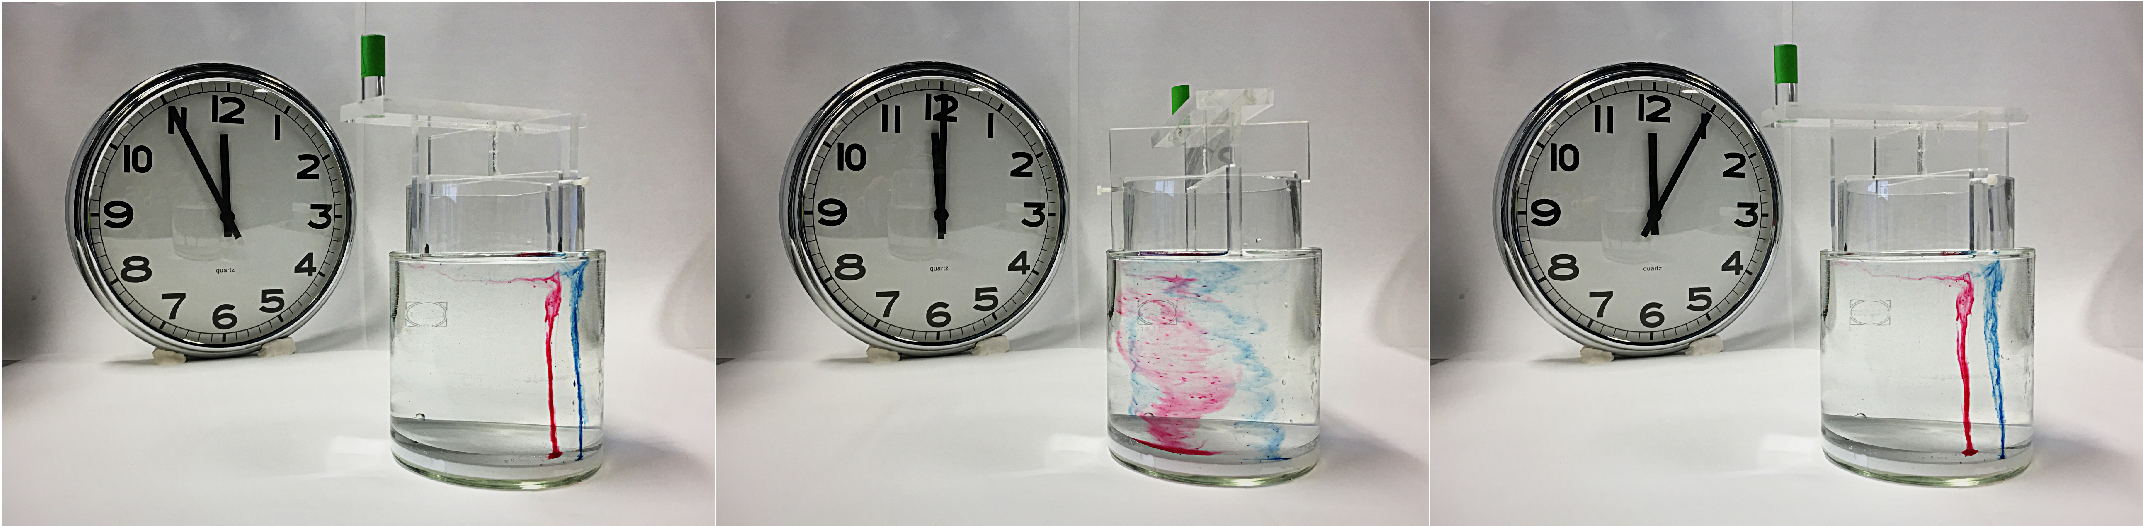
\includegraphics[width = 1\textwidth]{Slike/TaylorCouette}
	\caption{Zabaven eksperiment, pri katerem se v ozkem prostoru med dvema koncentričnima valjema nahaja viskozna tekočina, ki jo na dveh mestih označimo z liso barvila. Valja pet minut vrtimo v nasprotnih smereh (Stokesov tok, ki tako nastane, imenujemo Taylor-Couettov tok), da se lisi pomešata, nato smeri vrtenja obrnemo in po petih minutah se lisi ponovno sestavita. Pridobljeno iz  \cite{Wiki-StokesFlow}.}
	\label{fig:TaylorCouette}
	\vspace{-0.3cm}
\end{figure}

Sistem \texttt{PDE}, ki ga obravnavamo, zapišemo bolj jedrnato v matrični obliki. To je enostavno, če je sistem linearen. Uvedemo diferencialni operator $\mathbsf{A}$:
\begin{equation}
	\mathbsf{A}(\mathbf{x}) = \mathbsf{A}_0(\mathbf{x}) + \mathbsf{A}_1(\mathbf{x}) \frac{\pd}{\pd x_1} + \mathbsf{A}_2(\mathbf{x}) \frac{\pd}{\pd x_2} \ ,
\end{equation}

\setlength{\textheight}{26.4cm}
\pagebreak
\setlength{\topmargin}{1.6cm}			% Header Top Margin Height
\setlength{\headheight}{0.0cm}
\setlength{\headsep}{0.0cm}			% Header Lower Margin Height	 Footer height
\fancyhf{}
\fancyfoot[C]{\thepage}

s katerim lahko sistem enačb zapišemo kot:
\begin{IEEEeqnarray}{cc}
	\mathbsf{A}(\mathbf{x}) \cdot \mathbf{u}(\mathbf{x}) = \mathbf{f}(\mathbf{x}) \ . \label{eq:compactPDE} & \hspace{1.0cm} \texttt{jedrnat zapis PDE} \\[0.25cm]
	\left(\mathbsf{A}_0(\mathbf{x}) + \mathbsf{A}_1(\mathbf{x}) \frac{\pd}{\pd x_1} + \mathbsf{A}_2(\mathbf{x}) \frac{\pd}{\pd x_2}\right) \cdot \mathbf{u}(\mathbf{x}) = \mathbf{f}(\mathbf{x}) & \label{eq:matrixPDE1}
\end{IEEEeqnarray}
V matriko $\mathbsf{A}_0$ spravimo vse koeficiente pred členi z odvisnimi spremenljivkami, v matriko $\mathbsf{A}_1$ vse koeficiente pred členi z odvodi odvisnih spremenljivk po $x_1$ in v $\mathbsf{A}_2$ vse koeficiente pred členi z odvodi odvisnih spremenljivk po $x_2$. Ostale člene zložimo v vektor $\mathbf{f}$. Stokesove enačbe \eqref{eq:StokesDiv} - \eqref{eq:StokesCurl} lahko po zgledu enačbe \eqref{eq:matrixPDE1} zapišemo kot:
\begin{equation}
	\left[ \,
	\begin{pmatrix}
		0 & 0 & 0 & 0 \\
		0 & 0 & 0 & 0 \\
		0 & 0 & 0 & 0 \\
		0 & 0 & 0 & 1
	\end{pmatrix} +
	\begin{pmatrix}
		1 & 0 & 0 & 0 \\
		0 & 0 & 1 & 0 \\
		0 & 0 & 0 & -1 \\
		0 & -1 & 0 & 0
	\end{pmatrix} \frac{\pd}{\pd x} +
	\begin{pmatrix}
		0 & 1 & 0 & 0 \\
		0 & 0 & 0 & 1 \\
		0 & 0 & 1 & 0 \\
		-1 & 0 & 0 & 0 \\
	\end{pmatrix} \frac{\pd}{\pd y} \, \right]
	\ \cdot \
	\begin{pmatrix}
		u(\mathbf{x}) \\ v(\mathbf{x}) \\ p(\mathbf{x}) \\ \omega(\mathbf{x})
	\end{pmatrix}
	\ = \
	\begin{pmatrix}
		0 \\ f_1(\mathbf{x}) \\ f_2(\mathbf{x}) \\ 0
	\end{pmatrix} \ .
\end{equation}

\section{Temelji \texttt{LSFEM}}

Vse različice \texttt{FEM} vsaj okvirno temeljijo na variacijskem pristopu, kjer ne operiramo neposredno na \texttt{PDE}, ampak jih najprej pretvorimo v enakovreden variacijski problem: omislimo si \textbf{poskusno funkcijo} $\mathbf{w}(\mathbf{x})$, ki jo napnemo nad domeno $\Omega$, in izberemo funkcional $I[\mathbf{w}(\mathbf{x})]$, ki za vsako $\mathbf{w}(\mathbf{x})$ vrne neko realno število. Za uspešnost variacijskega pristopa moramo izbrati funkcional, ki vrne najmanjšo vrednost, ko je $\mathbf{w}(\mathbf{x})$ enaka rešitvi. Kadar obstaja s sistemom \texttt{PDE} povezan energijski potencial, je to fizikalno najintuitivnejša izbira za konstrukcijo funkcionala. Zato ni presenetljivo, da je bila \textbf{Rayleigh-Ritzeva različica} \texttt{FEM} (\texttt{RRFEM}), ki jo na tak način dobimo, razvita prva (temelji postavljeni 1909) \cite{RitzW-Variationsprobleme}. Konstrukcija funkcionala in njegova minimizacija sta tipična koraka variacijskega pristopa in nista specifična za \texttt{RRFEM}: vzamemo neko funkcijo poskusne funkcije $F\left(\mathbf{w}\right)$ in jo integriramo po domeni $\Omega$:
\begin{equation}
	I[\mathbf{w(x)}] = \int_{\Omega} F\left(\mathbf{w(x)}\right) \, \ud \Omega \hspace{1.4cm} \texttt{funkcional poskusne funkcije} \quad .
	\label{eq:GeneralFunctional}
\end{equation}
$F\left(\mathbf{w}(\mathbf{x})\right)$ je npr.\ pri \texttt{RRFEM} energijski potencial, dobljen funkcional pa skupna potencialna energija sistema. Rešitev $\mathbf{u}(\mathbf{x})$ potemtakem minimizira potencialno energijo sistema, zaradi česar \texttt{RRFEM} poseduje last\-nost najboljšega približka, hkrati pa vodi do sistema linearnih algebrajskih enačb, ki je zelo prikladen za reševanje s hitrimi iteracijskimi metodami. Različica metode se je izkazala pri reševanju problemov v gradbenem inženirstvu, kjer je s problemom vedno povezan energijski potencial. Večina računalniških programov s tega področja zato še danes temelji na \texttt{RRFEM}.

S \texttt{PDE} povezan energijski potencial žal vedno ne obstaja, kar velja predvsem v dinamiki tekočin. To je motiviralo razvoj Galerkinove različice \texttt{FEM} (\texttt{GFEM}), ki je zastavljena kot posplošitev \texttt{RRFEM}, a na precej neroden, ad hoc način. Akademiki so pričakovali, da se bo uspeh \texttt{RRFEM} v gradbenem inženirstvu ponovil v dinamiki tekočin z Galerkinovo metodo, vendar se to ni zgodilo \cite{JiangB-LSFEM}. Večina računalniških programov za simulacije dinamike tekočin je dandanes napisana na osnovi \texttt{GFEM}, saj je na svetu že lep čas (od 1940-ih) in je zanjo napisane ogromno literature. To ne velja za mlajšo \texttt{LSFEM}. Ideja \texttt{GFEM} je, da lahko za vsak sistem \texttt{PDE} definiramo vektor ostanka (glej enačbo \eqref{eq:compactPDE}):
\begin{equation}
	\mathbf{R(w(x))} = \mathbsf{A}(\mathbf{x}) \cdot \mathbf{w(x)} - \mathbf{f(x)} \hspace{1.3cm} \texttt{vektor ostanka .}
	\label{eq:residual}
\end{equation}
ki ga potem na nek način poskušamo minimizirati. To idejo uporabimo tudi pri \texttt{LSFEM}, kjer se minimizacije lotimo na legitimen način, preko funkcionala:
\begin{equation}
	\boxed{\, I[\mathbf{w(x)}] = \int_{\Omega} ||\mathbf{R(w(x))}||^2 \, \ud \Omega = \int_{\Omega}\mathbf{R \cdot R} \ \ud \Omega \,} \hspace{1.3cm} \texttt{funkcional LSFEM ,}
\end{equation}
kar pomeni, da minimiziramo vsoto kvadratov ostanka - od tod ime \emph{metoda najmanjših kvadratov}. Nadaljuj\-mo razlago preko splošnega funkcionala \eqref{eq:GeneralFunctional}, da bomo lahko kasneje orisali še postopek minimizacije pri \texttt{GFEM} in komentirali slabosti, ki jih prinese.

Ko smo torej prepričani, da ima funkcional \eqref{eq:GeneralFunctional} minimum pri rešitvi $\mathbf{u}(\mathbf{x})$, sledimo znanemu Euler-Lagrangevemu postopku. Ta nas pripelje do variacijske izjave, ki velja le, kadar je poskusna funkcija $\mathbf{w}(\mathbf{x})$ enaka rešitvi $\mathbf{u}(\mathbf{x})$. Poskusno funkcijo razvijemo okoli rešitve:
\begin{equation}
	\widetilde{\mathbf{w}}(\mathbf{x}, \varepsilon) = \mathbf{u}(\mathbf{x}) + \varepsilon \mathbf{v}(\mathbf{x}) \ ,
	\label{eq:trialFuncAroundSol}
\end{equation}
kjer je $\mathbf{v}(\mathbf{x})$ poljubna odmična funkcija, $\varepsilon$ pa realno število. Razvoj \eqref{eq:trialFuncAroundSol} vstavimo v funkcional \eqref{eq:GeneralFunctional} namesto $\mathbf{w}(\mathbf{x})$ in odvajamo po $\varepsilon$:
\begin{equation}
\frac{\ud I}{\ud \varepsilon} = \int_{\Omega} \frac{\ud}{\ud \varepsilon} F(\widetilde{\mathbf{w}}) \, \ud \Omega = \int_{\Omega} \frac{\ud F}{\ud \widetilde{\mathbf{w}}} \cdot \frac{\ud \widetilde{\mathbf{w}}}{\ud \varepsilon} \ \ud \Omega = \int_{\Omega} \frac{\ud F}{\ud \widetilde{\mathbf{w}}} \cdot \mathbf{v} \ \ud \Omega \ .
\label{eq:funcDerivative}
\end{equation}
Kadar gre $\varepsilon$ proti nič, gre $\widetilde{\mathbf{w}}(\mathbf{x}, \varepsilon)$ proti rešitvi problema $\mathbf{u}(\mathbf{x})$, hkrati pa vemo, da ima funkcional $I$ pri $\mathbf{u}(\mathbf{x})$ minimum. Da dobimo \textbf{variacijsko izjavo}, torej odvod funkcionala \eqref{eq:funcDerivative} enačimo z nič in potem $\varepsilon$ pošljemo proti nič:
\begin{equation}
	\lim_{\varepsilon \rightarrow 0} \frac{\ud I}{\ud \varepsilon} = \lim_{\varepsilon \rightarrow 0} \int_{\Omega} \frac{\ud F(\widetilde{\mathbf{w}}(\mathbf{x}, \varepsilon))}{\ud \widetilde{\mathbf{w}}} \cdot \mathbf{v(\mathbf{x})} \ \ud \Omega = \ \boxed{\, \int_{\Omega} \left( \lim_{\varepsilon \rightarrow 0} \frac{\ud F(\widetilde{\mathbf{w}})}{\ud \widetilde{\mathbf{w}}} \right) \cdot \mathbf{v} \ \ud \Omega = 0 \ , \quad \forall \mathbf{v(\mathbf{x})}\, \vphantom{\Biggr{)}}} \ .
\end{equation}
Komaj tukaj se začne formulacija Galerkinove različice. Na izraz v oklepaju gledamo v kontekstu \texttt{RRFEM} kot na neko funkcijo potenciala povezanega s sistemom \texttt{PDE}. Namesto omenjenega izraza v oklepaju vstavimo vektor ostanka \eqref{eq:residual}:
\begin{equation}
	\int_{\Omega} \mathbf{R(w(x))} \cdot \mathbf{v(x)} \ \ud \Omega = 0
\end{equation}
in upamo, da bo novi način minimiziral ostanek $\mathbf{R}$. Poskusno funkcijo  Pristop imenujemo \emph{metoda uteženih ostankov (method of weighted residuals)}. Od te točke dalje nadaljujemo z diskretizacijo problema, to je, pretvorbo na sistem $N$ algebrajskih enačb. Ta korak je enak pri vseh različicah \texttt{FEM}

Potem omejimo Diskretizacija problema 

Galerkin, Najmanših kvadratov \cite{JiangB-LSFEM}
Basic lemma of variational principles: Temeljni lema variacijskih načel.

\textbf{Rayleigh-Ritzeva različica} \texttt{FEM}, ki je bila razvita prva in ima korenine v začetku dvajsetega stoletja (cite), je prav tako variacijska metoda.